\documentclass[12pt, a4paper]{article}

\usepackage[utf8]{inputenc}
\usepackage[T1]{fontenc}
\usepackage[brazilian]{babel}
\usepackage{mathptmx}
\usepackage{amsmath, amssymb}
\usepackage{graphicx}
\usepackage{booktabs}
\usepackage{geometry}
\usepackage{float}
\usepackage{setspace}
\usepackage{caption}

\geometry{top=3cm, bottom=2cm, left=3cm, right=2cm}
\setstretch{1.5}
\captionsetup{font=small, labelfont=bf, labelsep=endash}

\begin{document}

\begin{center}
    \Large\textbf{Relatório Intermediário de Benchmarking -- Cenário 2} \\[0.2cm]
    \large\textit{Avaliação de Desempenho: 4 Núcleos e Armazenamento Fragmentado} \\[0.5cm]
    \normalsize\textbf{Projeto DataOps / UNIFEI} \\
    \small{\today}
\end{center}

\vspace{0.5cm}
\noindent\rule{\textwidth}{1pt}

\section*{1. Descrição do Cenário}
Este documento retrata a segunda fase dos testes de escalabilidade vertical do ecossistema Apache Druid. Comprovado o estrangulamento sistêmico no Cenário 1 (onde apenas 2 núcleos geraram latências de 4.600 ms), o \textit{cluster} foi reconfigurado via \textit{Docker Compose Override}. Alocaram-se \textbf{4 núcleos lógicos totais} (2 \textit{threads} distribuídas para o nó \textit{Broker} e 2 para o nó \textit{Historical}), dobrando assim o poder de fogo paralelizado.

Nesta etapa, o objetivo central foi avaliar o impacto puro do incremento de CPU, mantendo-se inalterada a patologia de armazenamento: os $\sim$211 MB de metadados permanecem distribuídos em \textbf{6.518 minúsculos arquivos (Tiny Segments)}.

\section*{2. Ganhos de Escala vs. O Paradoxo Contínuo}
Os resultados expressos na Tabela 1 demonstram a eficácia da natureza multithread do banco colunar. O aumento de CPU praticamente cortou pela metade a ineficiência de varredura. Consultas complexas que orbitavam em $\sim$4.600 ms despencaram para o patamar seguro de \textbf{2.000 ms a 2.900 ms} em leituras \textit{Cold Start}.

\begin{table}[H]
\centering
\caption{Resultados do Cenário 2 - CPU Intermediária (4 Cores)}
\vspace{0.2cm}
\begin{tabular}{@{}lcccc@{}}
\toprule
\textbf{Domínio da Consulta SQL} & \textbf{Cold (ms)} & \textbf{Warm (ms)} & \textbf{Otimização} & \textbf{Registros} \\
\midrule
    Bench 1 Serie Temporal & 2993.05 & 1957.83 & 34.59\% & 100 \\
    Bench 2 Alta Cardinalidade & 2611.78 & 2130.59 & 18.42\% & 50 \\
    Bench 3 Filtros Complexos & 2113.30 & 1970.01 & 6.78\% & 9 \\
    BI 1 ONS Infraestrutura & 2170.75 & 2123.40 & 2.18\% & 15 \\
    BI 2 FUNAI Terras Indigenas & 1994.80 & 2023.17 & -1.42\% & 10 \\
    BI 3 Defesa Civil Risco & 2034.59 & 1969.18 & 3.21\% & 81 \\

\bottomrule
\end{tabular}
\end{table}

Contudo, a constatação científica de maior peso reside na \textbf{ineficiência persistente do Cache}. Apesar da melhoria nos tempos globais, a consulta ``BI\_2 FUNAI'' ainda assinalou otimização negativa (-1.42\%), ou seja, o \textit{Warm Start} demorou mais que o acesso direto aos discos. Isto comprova que injetar processador ameniza a latência geral, mas \textbf{não soluciona o I/O Overhead} (custo de roteamento e fusão em RAM) decorrente de 6.518 blocos estilhaçados.

\begin{figure}[H]
\centering
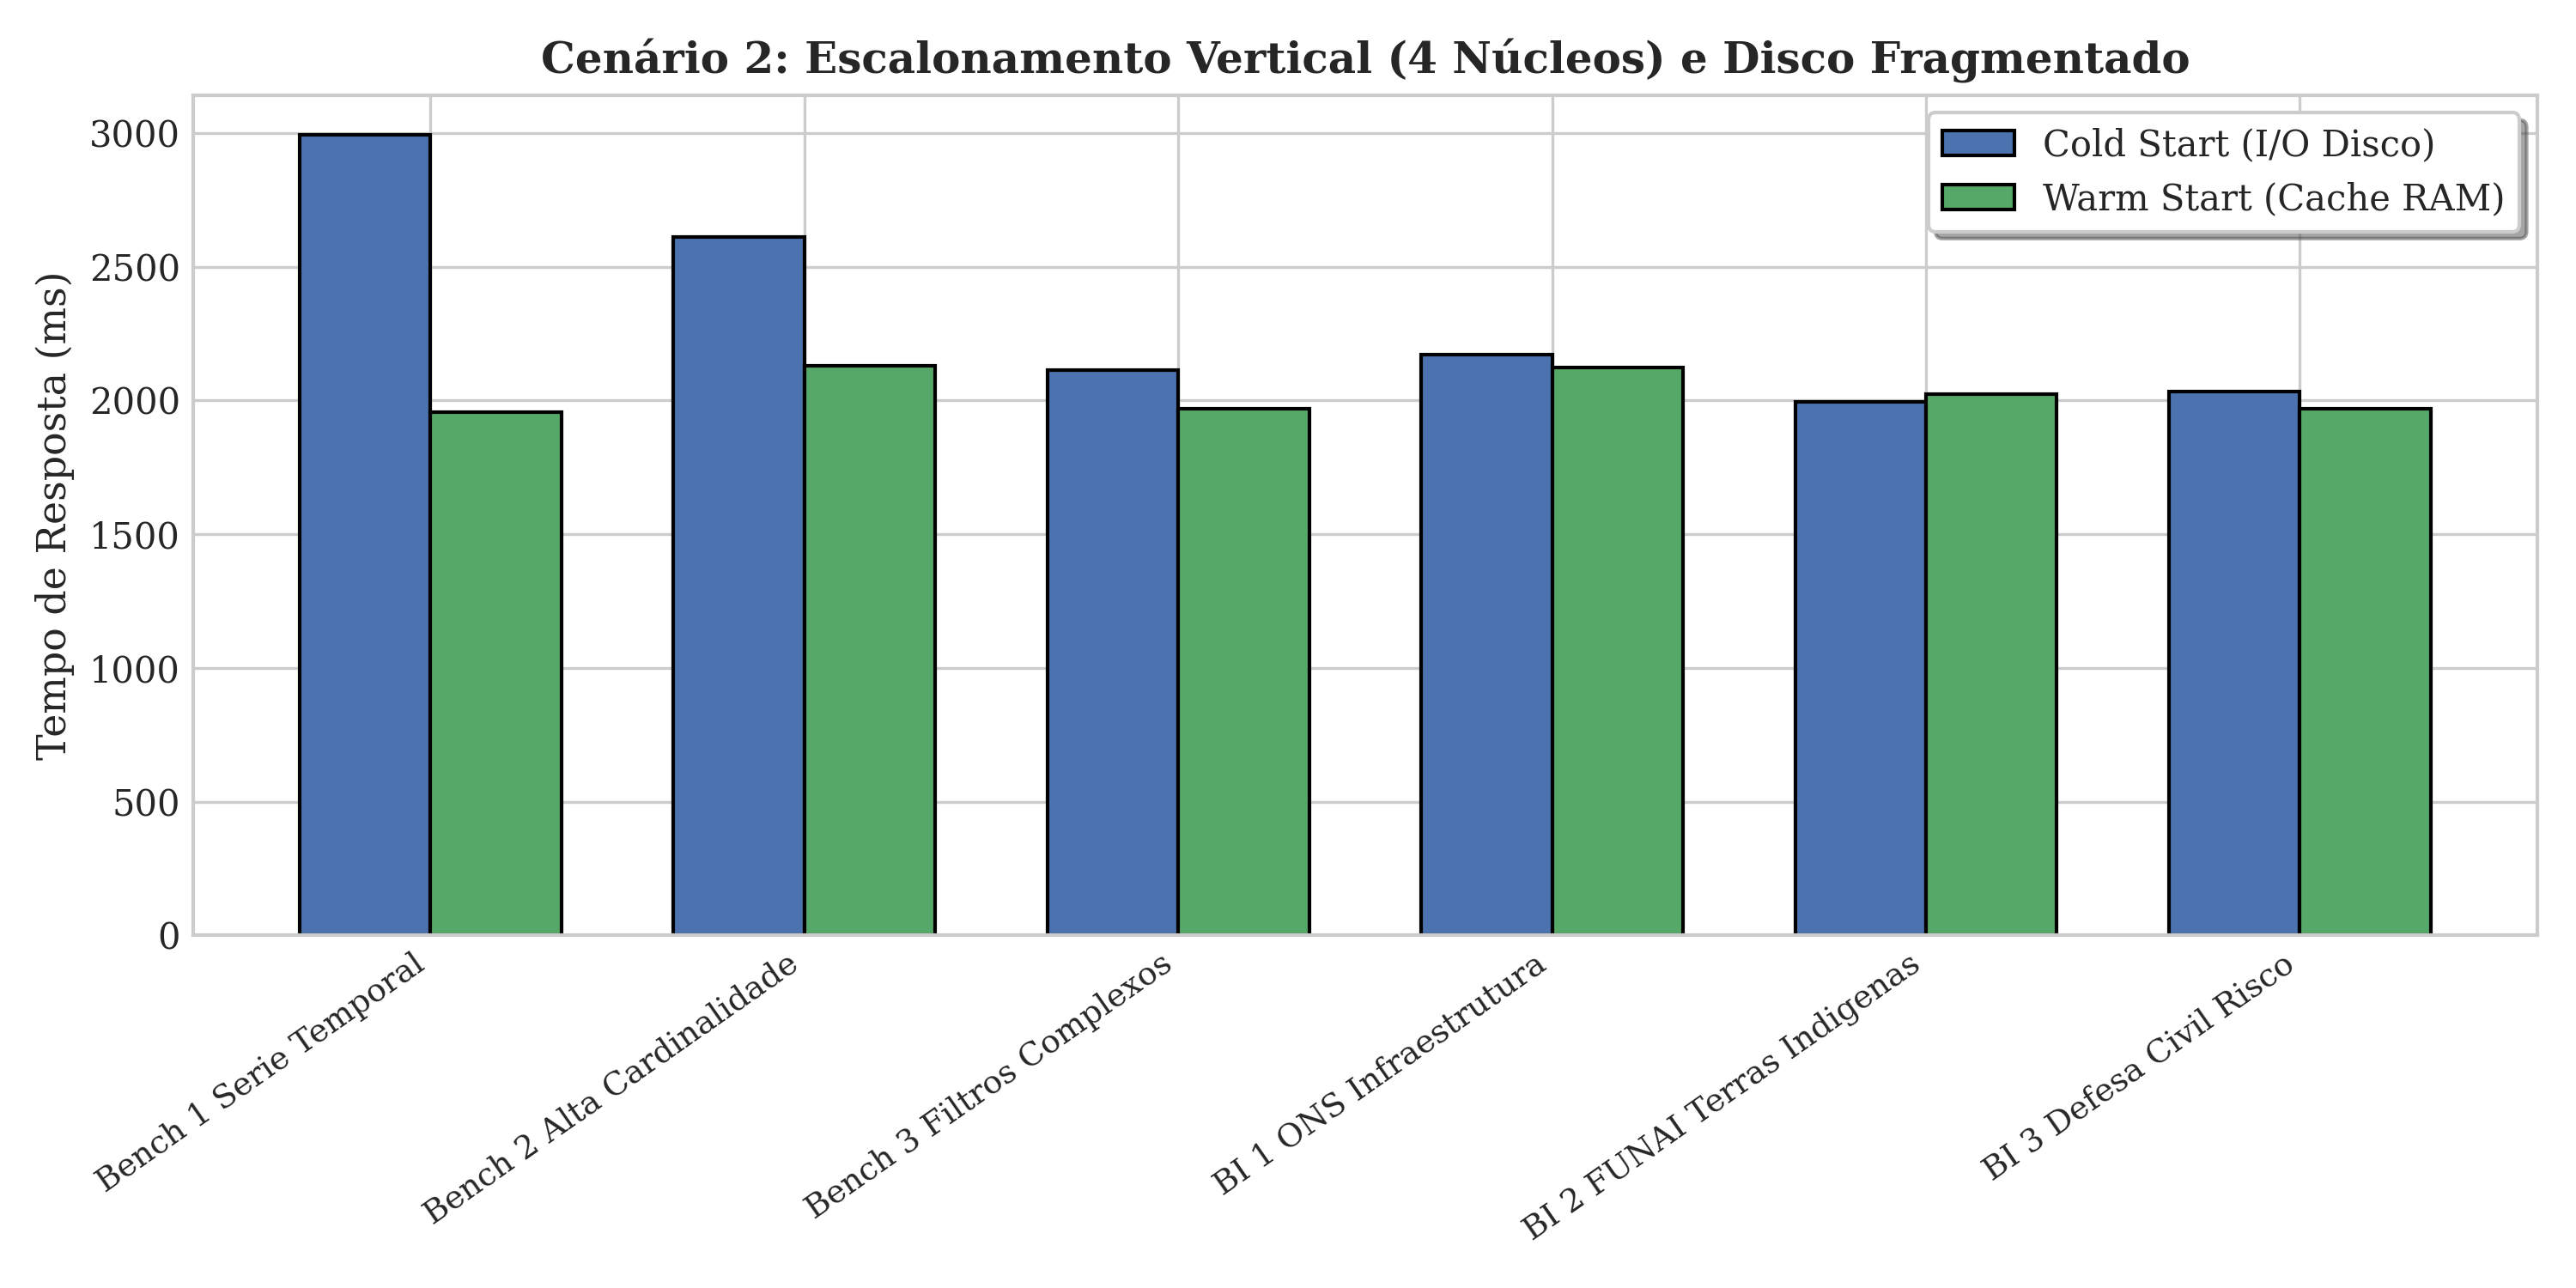
\includegraphics[width=0.9\textwidth]{fig_desemp_cenario2.png}
\caption{Comparativo atestando ganhos escalares, mas evidenciando falhas de Warm Start.}
\end{figure}

\begin{figure}[H]
\centering
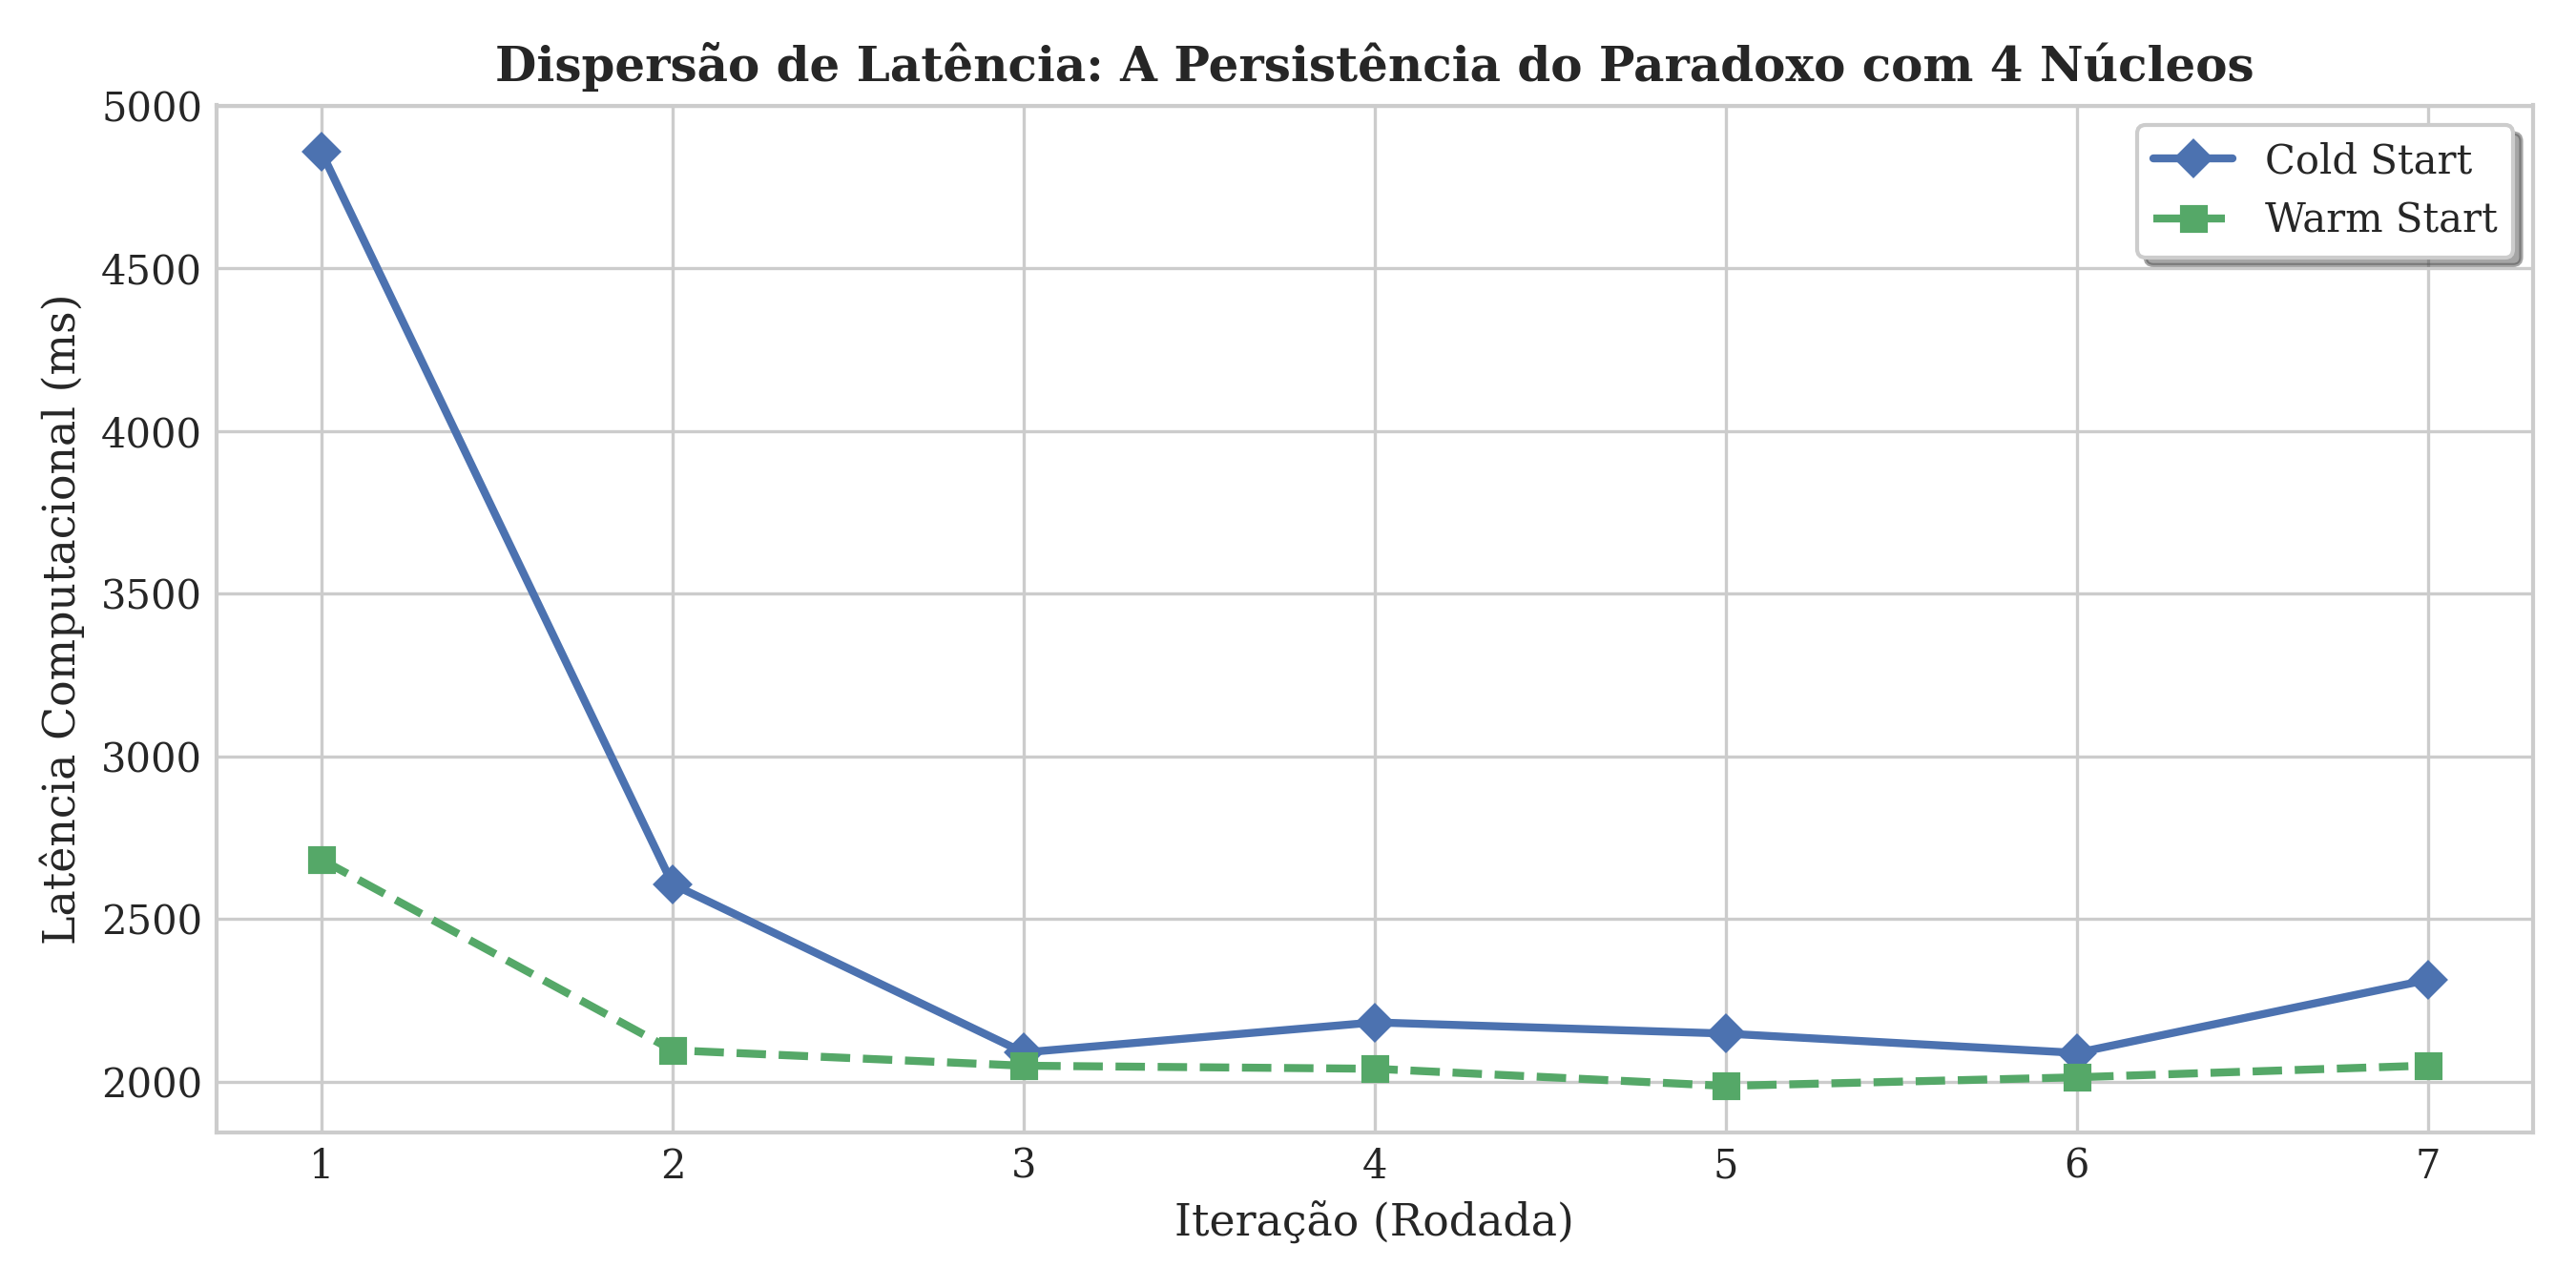
\includegraphics[width=0.8\textwidth]{fig_var_cenario2.png}
\caption{Dispersão refletindo a disputa da ULA no gerenciamento da base não compactada.}
\end{figure}

\section*{3. Considerações e Próximos Passos}
A duplicação de núcleos validou o princípio de escalabilidade teórica, mas escancarou que motores OLAP são visceralmente dependentes da geometria dos dados. O último teste desta fase arquitetural (Cenário 3) levará a máquina ao limite físico (6 núcleos) antes que se aplique a resolução mandatória de \textit{DataOps}: a Compactação dos Segmentos.

\end{document}
